
\chapter{Umsetzung}

\section{Architektur}
Die Architektur des Projekts umfasst folgende Komponenten:
\begin{enumerate}
    \item \textbf{Virtuelles Netzwerk:} Ein Azure Virtual Network mit Subnetzen für die Anwendung und die Datenbank.
    \item \textbf{Datenbank:} Eine PostgreSQL Flexible Server Instanz, die als PaaS-Dienst bereitgestellt wird.
    \item \textbf{Webanwendung:} Mehrere virtuelle Maschinen (VMs) mit einer Load Balancer-Konfiguration, die eine Next.js-Anwendung hosten.
    \item \textbf{Monitoring:} Eine Monitoring Instanz über die mittels pgAdmin, Prometheus und Graphana die Überwachung der Anwendung erfolgt.
    \item \textbf{Automatisierung:} Terraform wird verwendet, um die Infrastruktur zu erstellen, und Ansible, um die VMs zu konfigurieren und die Anwendung bereitzustellen.
\end{enumerate}

\begin{figure}[H]
    \centering
    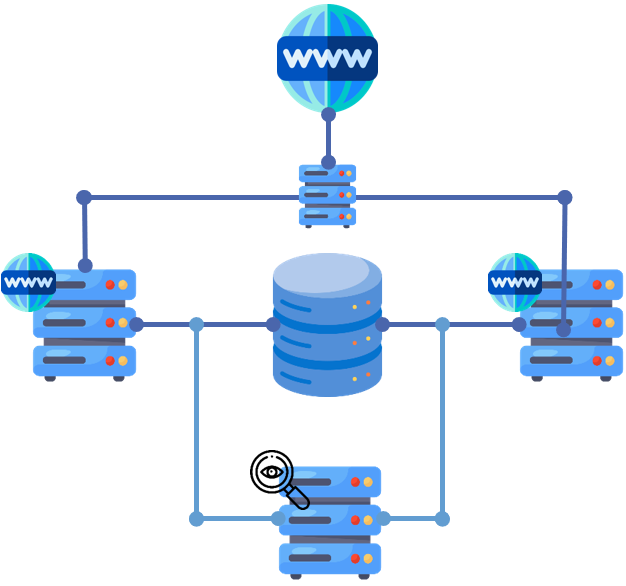
\includegraphics[width=0.6\textwidth]{resources/images/Architektur.png}
    \caption{Architektur des Projekts}
\end{figure}

\section{Aufbauablauf}

\subsection*{Schritt 1: Infrastruktur mit Terraform}
Zunächst wird die Infrastruktur mit Terraform bereitgestellt. Dazu wird eine Azure Resource Group erstellt, die als Container für alle Ressourcen dient. Anschließend wird ein virtuelles Netzwerk mit Subnetzen für die Anwendung und die Datenbank konfiguriert. Eine PostgreSQL Flexible Server Instanz wird mit privatem Netzwerkzugriff eingerichtet. Danach werden zwei virtuelle Maschinen für die Webanwendung erstellt und mit einem Load Balancer verbunden. Abschließend wird ein Monitoring-Server bereitgestellt, um die Überwachung der Anwendung zu ermöglichen.

\subsection*{Schritt 2: Konfiguration mit Ansible}
Konfiguration der App VMs
\begin{itemize}
    \item Installation von Node.js und PostgreSQL-Client auf den VMs.
    \item Bereitstellung der Next.js-Anwendung aus dem Git-Repository.
    \item Konfiguration der Umgebungsvariablen für die Datenbankverbindung.
    \item Erstellung eines Systemd-Dienstes, um die Anwendung automatisch zu starten.
\end{itemize}

Konfiguration des Monitoring Servers
\begin{itemize}
    \item Installation von pgAdmin, Prometheus und Grafana auf dem Monitoring Server.
    \item Konfiguration von pgAdmin zur Verwaltung der Datenbank.
    \item Konfiguration von Prometheus und Grafana zur Überwachung der Anwendung.
    \item Einrichtung von Dashboards in Grafana zur Visualisierung der Metriken.
\end{itemize}
